%%%%%%%%%%%%%%%%%%%%%%%%%%%%%%%%%%%%%%%%%%%%%%%%%%%%%%%%%%%%%%%%%%%%%%%%%%%%%%%%%%%%%%%%%%%%%%%%%%%%%%%%%%%%
\section{Introduction}

Sketch-based interfaces provide an intuitive way to create and explore three-dimensional shapes~\cite{sketchbasedmodelingsurveycg2009}. Most shapes of interest can be drawn, and most humans grow up with at least rudimentary drawing skills~\cite{DeckerChildren1988}. Most humans cannot, however, draw very well. Hence, sketch-based interfaces need to interpret a crude drawing and map it to a detailed shape. \st{Typically, this is done in a data-driven manner} \hl{This problem could be tackled in a data-driven manner}: each sketched component is used to search a repository for a high-quality shape with a matching part, which can be extracted and incorporated into the design.

\begin{figure}[h!]
\centering
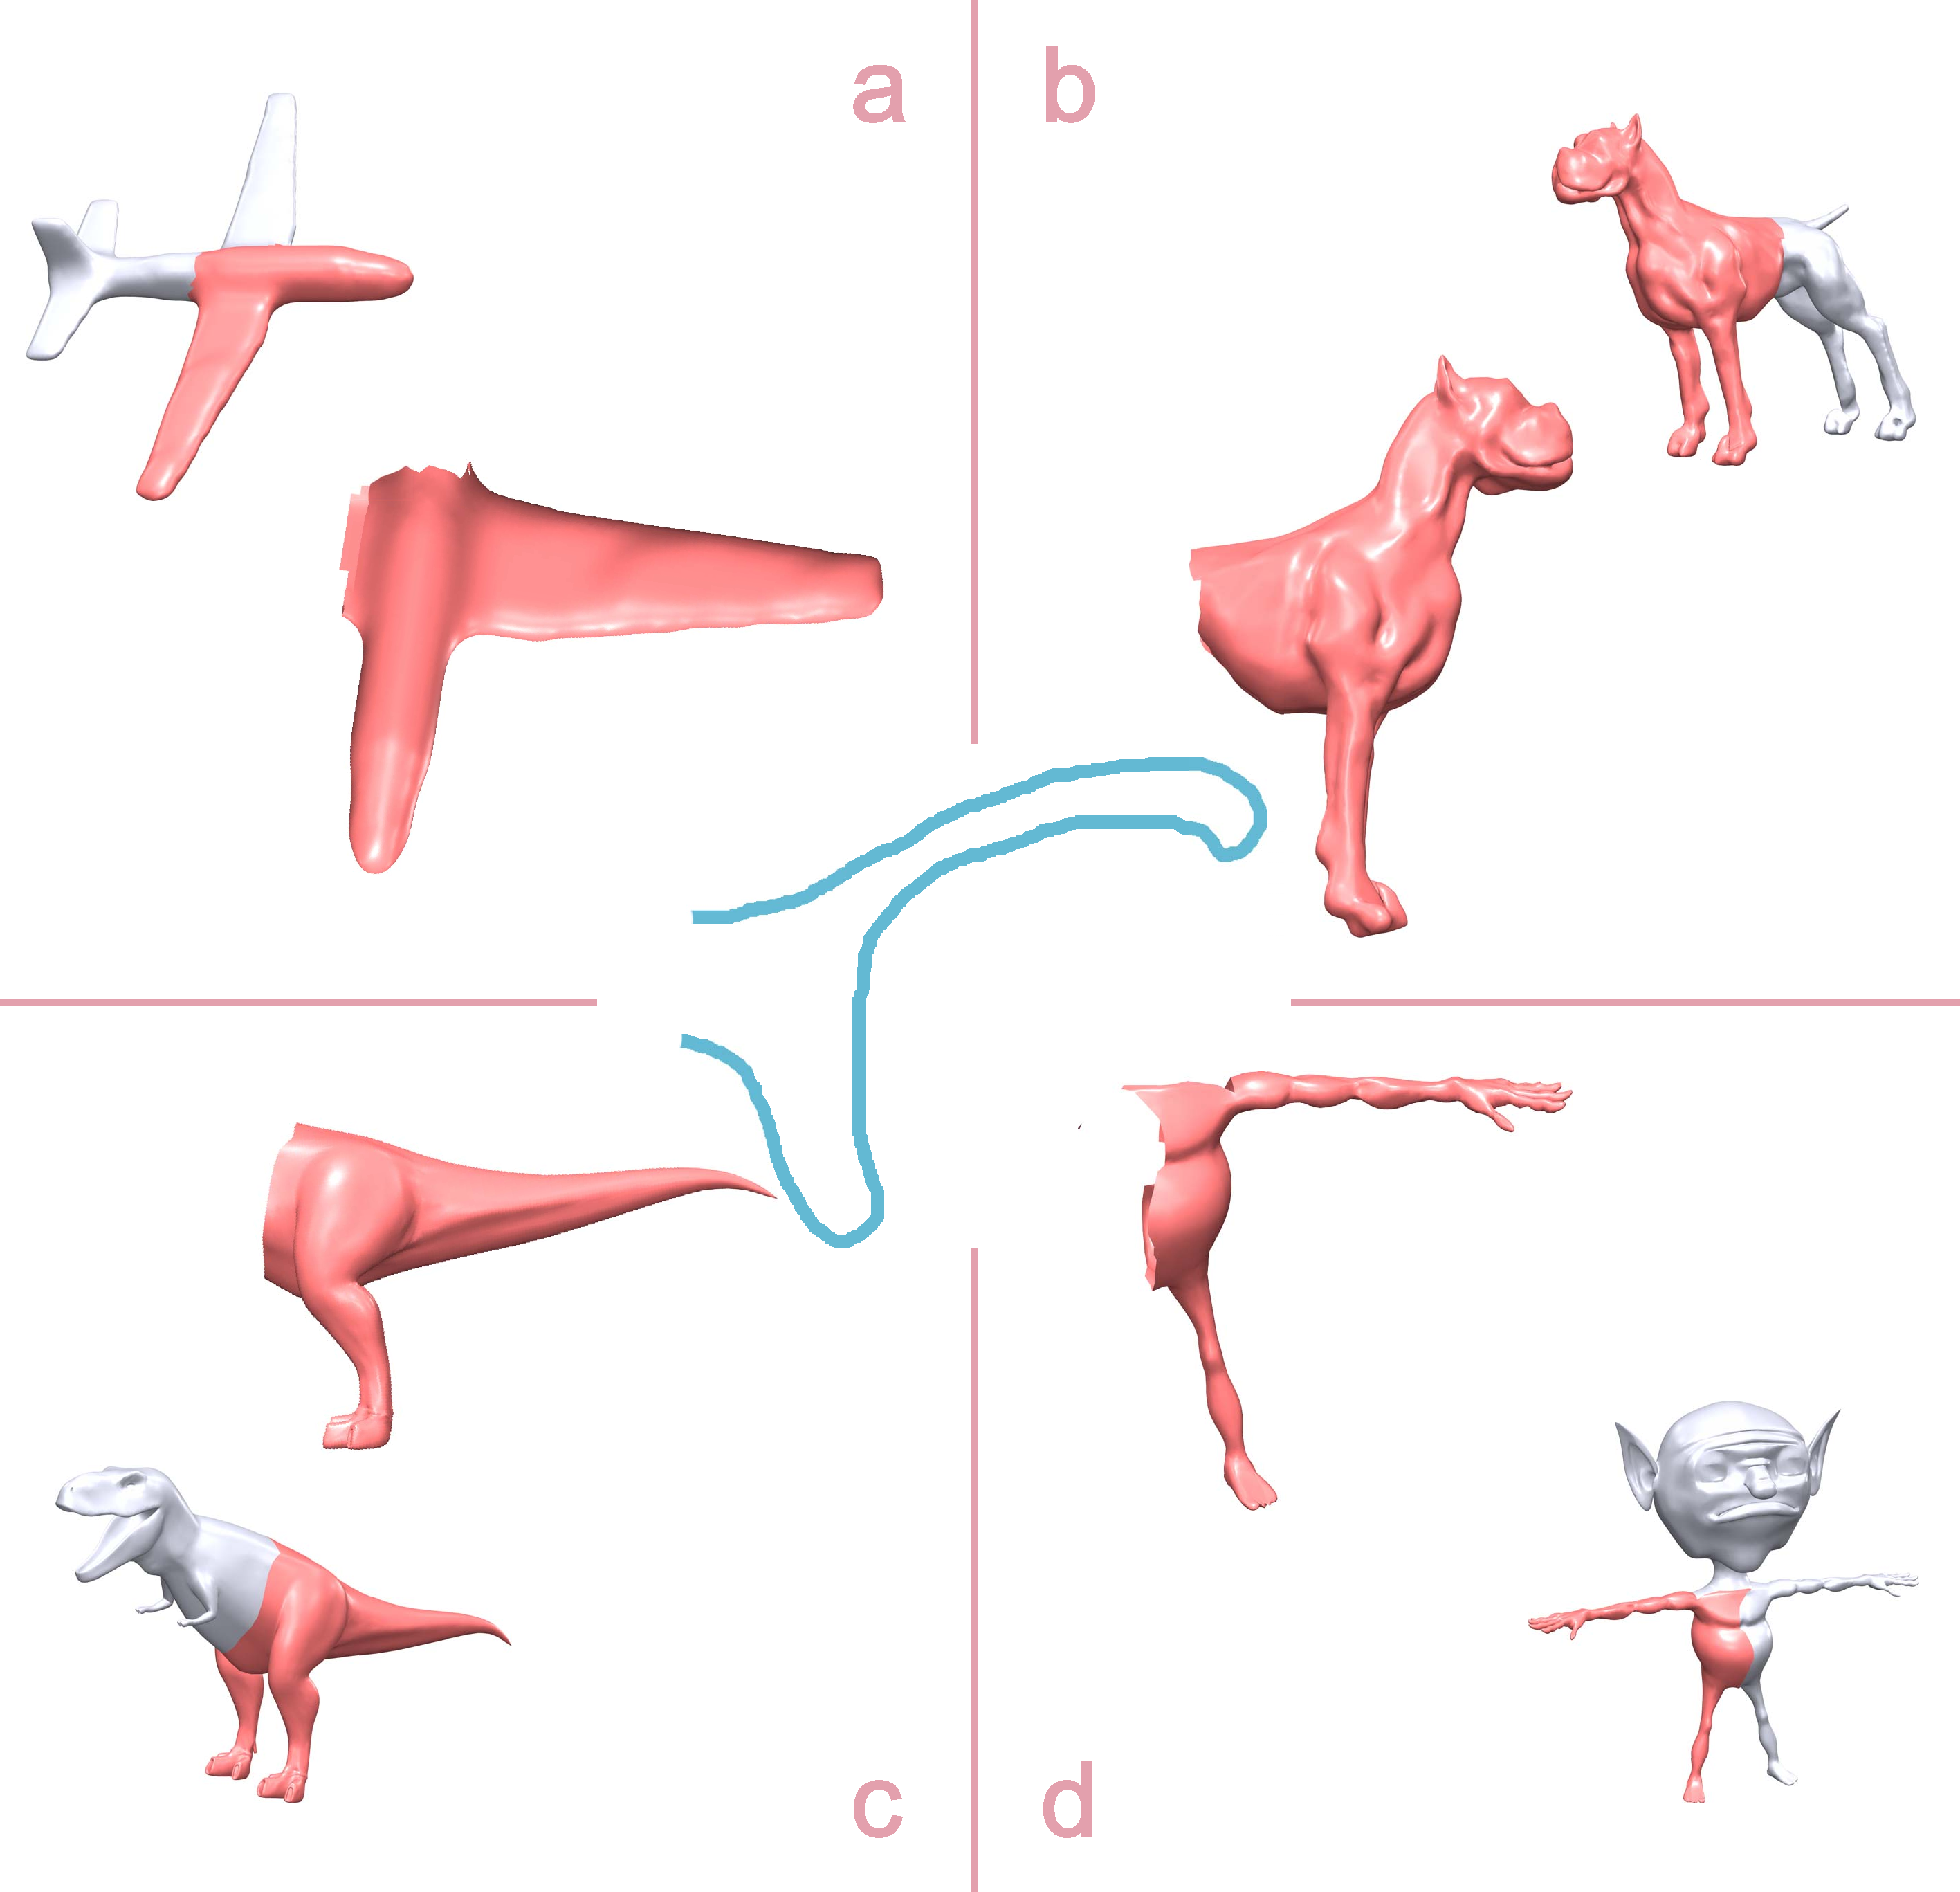
\includegraphics[width=0.9\linewidth]{./Material/TeaserSGP.pdf}
\caption{Given a roughly drawn sketch, our algorithm rapidly searches a shape database to identify and extract customized parts that match the sketch. No presegmentation is required: the retrieved parts can be irregular and not match any standard segmentation.}
\label{fig:HeadPic}
\end{figure}

\begin{figure*}[t]
\centering
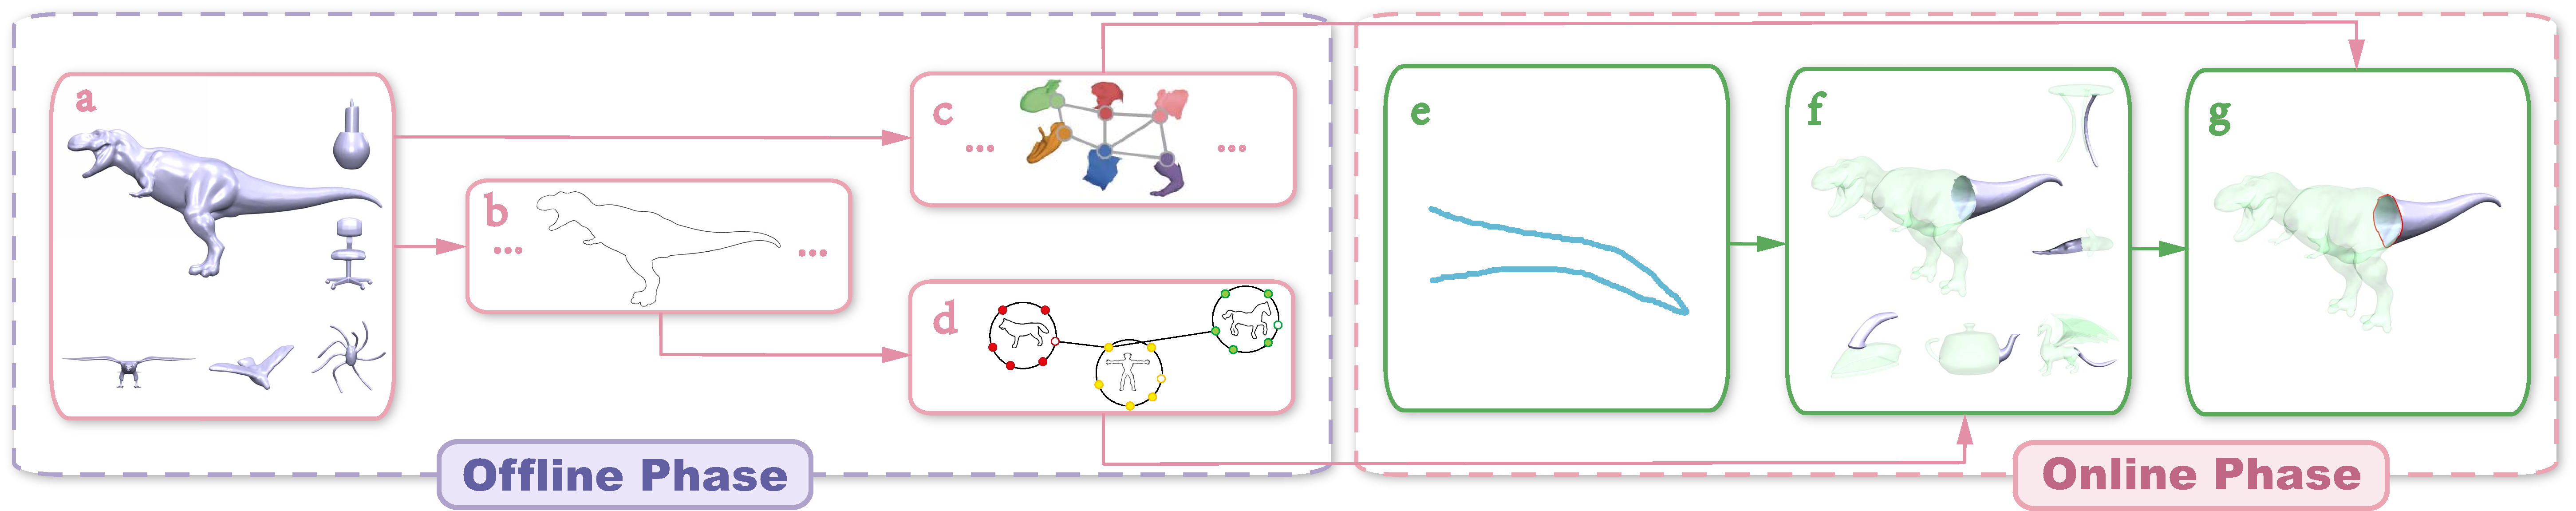
\includegraphics[width=\linewidth]{./Material/Pipeline.pdf}
\caption{Pipeline of our system. In the offline phase, for each model in a given shape database (a), we first extract its boundary contours (b). We then construct the \textbf{super-face graph} for each model (c), and organize the boundary contours of all models into a \textbf{randomized compound $k$-NN graph} (d). In the online phase, the user draws a rough sketch to convey his/her design intent (e). Regions of database shapes matching the sketch are rapidly identified via partial shape matching (f). A selected part is further refined to optimize its boundary and better match the sketch (g)}\label{fig:pipeline}
\end{figure*}

Matching a sketched component to a shape database is a challenging partial matching problem. In the general setting, an arbitrary region of the shape may match the sketch. To reduce the complexity, existing methods leverage a prior segmentation of each shape into predefined semantic parts~\cite{sketchbasedcompositionfunkhousersbim2008,sketchtodesignxukaicgf2013}. These parts are individually matched to the sketch, reducing the problem to one of global, rather than partial matching~\cite{EitRicBouHilAle12}.

In this paper, we present {\ProjName}, a new end-to-end technique for sketch-based customized part extraction. In contrast to prior work, we require no prior segmentation of the database shapes into predefined parts. Instead, we perform {\em on-demand} segmentation of retrieved database shapes, to accurately fit the user intent expressed in the sketched stroke (Figure \ref{fig:HeadPic}). This significantly expands the design space available to the user and enables several applications.

Designing such an algorithm presents hard technical challenges. Since a presegmented (or prelabeled) database is not available to us, we must simultaneously identify and extract parts that match sketched strokes, resulting in a potentially infinite search space. To prune this search space to a manageable size, we design a strategy to carefully balance between returning all possible matches, and providing an overly narrow set of matches. Further, the matching scheme must be fast enough so that appropriate candidate parts can be sought interactively. To address this challenge, we take a projective approach and turn the 3D partial matching problem into a 2D contour-based one. The 2D contours of all database shapes are segmented into fragments and organized based on fragment similarity, using an efficient data structure. Given a query sketch, our method can leverage the structure to quickly return all potentially matched parts via contour matching and match propagation.

Our paper has two main technical contributions, which together form the core of our algorithm:
\begin{itemize}
\setlength{\itemsep}{3pt}
\setlength{\parskip}{0pt}
\setlength{\parsep}{0pt}
\item A fast, sketch-based, partial 3D shape matching method based on multi-view projections. The projections are interlinked by matching fragments across different shapes, based on a novel randomized compound $k$-NN graph representation.
\item A novel customized segmentation method based on a super-face graph. The method quickly extracts candidate parts conforming to a user's sketch from a matched shape. The extraction employs a coarse-to-fine strategy to progressively refine part boundaries down to the level of individual faces.
\end{itemize}
